%% Format in ApJ style
\documentclass[iop]{emulateapj}
\usepackage{graphicx}
\setcounter{secnumdepth}{3}

\begin{document}

%% Title
\title{Observations of the Type IIn SN J13522411}

%% Authors and affiliations
\author{Ryan Hofmann and Nathan Smith}
\affil{Steward Observatory, University of Arizona}

%% Abstract
\begin{abstract}
We present visible and near-IR photometry and spectra of the type IIn supernova PSN J13522411. The light curve, though poorly sampled, indicates a peak $<50$ days after discovery around $M = -17$, followed by a slow decline. Spectra show strong hydrogen and helium emission that peaks $\sim200$ d after discovery, with a P-Cygni profile that becomes more absorptive as time progresses. We estimate the CSM has a radius of $\sim90$ AU and was ejected $<12$ yr before the explosion, with the velocity of the CSM implying a red or yellow supergiant as the progenitor. From the light curve, we estimate the total radiated energy to be $\sim10^{50}$ erg. Further details of the explosion will be determined as time allows.
\end{abstract}

%% Introduction
\section{Introduction} \label{intro}
Understanding the explosive deaths of massive stars as supernovae is an important area of astrophysical research, as it is through this process that heavy elements are formed and dispersed into the interstellar medium. One of the more interesting aspects of these phenomena, and one that is still not well understood, is how supernovae interact with their environments. A striking example of this interaction is the class SNe IIn, which have narrow emission lines and slowly declining light curves \citep{Fil97}.

Most of the peculiar features of SNe IIn can be explained by a shell of dense circumstellar material ejected from the star before it exploded. Initially, intense UV- and X-ray radiation from the explosion photoionize the slow-moving CSM, producing narrow-line emission with a Lorentzian profile. Later, the rapidly expanding shock collides with the CSM, causing broad emission with a line profile that depends on the distribution of the CSM.

There are two main ways that a star may develop a dense CSM before it explodes. The first, and arguably simplest, origin is a dense stellar wind, which is usually driven by very high luminosity, as in Wolf-Rayet stars, and/or by high opacity in the outer layers of the star, as would be expected in a red supergiant. In the case of Wolf-Rayet stars, this wind typically blows at hundreds or even thousands of kilometers per hour, effectively peeling away the star's outer layers; if the density of the stellar wind is relatively low, these stars will explode as type Ib or Ic SNe. Whereas in the case of red supergiants, the stellar wind may only blow at 100 km/s or less, but the density can be much greater; these stars, without a dense CSM, would typically explode as type IIL or IIP SNe.

The second method of producing a dense CSM is in bursts, typically eruptions driven by the complex internal dynamics of the star as it burns heavier elements. One of the best known instances of a star undergoing such eruptions would be the luminous blue variable (LBV) Eta Carinae, which erupted in 1841 and briefly became the second-brightest star in the sky. Today, we see the remnants of that eruption as a huge bipolar nebula called the Homunculus.

There is a third mechanism for creating a substantial CSM, and that is by shedding angular momentum, either from a rapidly rotating single star or from the merger of a binary. One well-known example of this is SN 1987A, the progenitor of which was determined to be a blue supergiant. More than ten years after the explosion, the shock wave began colliding with a dense ring of material which was shed $\sim20,000$ years ago \citep{Fra15}. As the expanding shock moves through and interacts with the ring and the surrounding CSM, it will reveal details of the mass loss history of the progenitor that will hopefully help to determine whether the ring originated in the single or binary model. It is unknown whether such structures are common for massive stars, as 1987A is one of only a handful of SNe to be continuously monitored for many years after the explosion; most SNe are in distant galaxies, and thus become too faint to observe in this manner. Had 1987A exploded in a distant galaxy, we might never have known about the ring of CSM and its implications. Likewise, if it had exploded just a few years after the ring was produced, 1987A might have been classified as a type IIn SN. For this and other reasons, SNe IIn are a complex and varied class of objects with a wide range of histories, and every instance is unique and worth careful analysis.

In this paper, we present visual and near-IR photometry and spectroscopy of PSN J13522411 from discovery up to $\sim450$ d afterward. PSN J13522411 was discovered by Zhangwei Jin and Xing Gao on 2015 Jan. 14.9 in three unfiltered images of NGC 5337. The reported apparent magnitude was 16.9, which we assume to be equivalent to the R magnitude, but is more likely to be an upper limit. No source was visible in images taken on Jan. 07 (limiting mag 19.5). It was classified as having a type IIn spectrum on 2015 Jan. 16.9 by Jujia Zhang and Xiaofeng Wang. At a redshift of $z = 0.007007$ (2165 km/s), this corresponds to a distance of 36.39 Mpc ($m - M = 32.8$ mag), with a Milky Way line-of-sight extinction $A_v = 0.038$ mag and reddening $E(B - V) = 0.013$ mag. PSN J13522411 resides in the outer disk of NGC 5337, at a projected separation of $\sim18$ arcsec ($\sim3$ kpc) from the host galaxy's nucleus. Our observations are presented in Section 2, and the light curve and spectral evolution are analysed in Section 3. Section 4 provides a summary of our work.

%% Observations
\section{Observations} \label{obs}

\begin{figure}
  \includegraphics[width=\linewidth]{graphics/Kuiper_R.jpeg}
  \caption{R-band image of NGC 5337 taken on 2016 March 17 with the Kuiper 61-inch telescope. PSN J13522411 is indicated by the arrow. The repeating vertical lines are bad columns.}
  \label{fig:kuiper}
\end{figure}

\subsection{Discovery} \label{obs:disc}
PSN J13522 was discovered on three 40-s survey images taken by Xing Gao in Xingming Observatory with an unfiltered CCD on a Celestron C14 Schmidt-Cassegrain telescope. The object first appeared on Jan. 09.9, and was confirmed on Jan. 14.9; nothing was visible in images taken on Jan. 07 (limiting mag 19.5).

\subsection{SLOTIS photometry} \label{obs:slotis}
After discovery of PSN J13522, the field was added to the queue of the robotic Super-LOTIS 24-inch telescope \citep[SLOTIS;][]{Wil08} on Kitt Peak for multifilter (B, V, R, and I) follow-up observations. Seeing varied between $\sim2-4$ arcsec. Images were automatically calibrated using a custom pipeline by Peter Milne, and aperture photometry was performed manually. The magnitudes were calibrated using the reference star list from the SLOTIS pipeline, shown in Table 4. The photometry is summarized in Table 1.

\subsection{UKIRT JHK photometry} \label{obs:ukirt}
Three sets of JHK images were collected during the same period as the SLOTIS data, using the UK Infrared Telescope's (UKIRT) Wide Field Camera instrument \citep[WFCAM;][]{Hod09}. The 'seeing', estimated from the full width at half-maximum intensity (FWHM) of stars on the CCD frame, varied between $\sim1-2$ arcsec. Aperture photometry was performed manually, and the magnitudes were calibrated using the same reference stars from SLOTIS. The results are summarized in Table 2.

\subsection{Kuiper BVR photometry} \label{obs:kuiper}
One set of images was recorded at a late time using the Mont4k CCD on the 61" Kuiper telescope on Mt. Bigelow \citep{Fon14}. Seeing was $<0.5$ arcsec. The R-band image with compass and scale is shown in Fig. \ref{fig:kuiper}. Aperture photometry was performed manually. Some of the reference stars were outside the field of view or saturated, and were thus excluded from the reduction. The results are summarized in Table 3.

\begin{figure}
  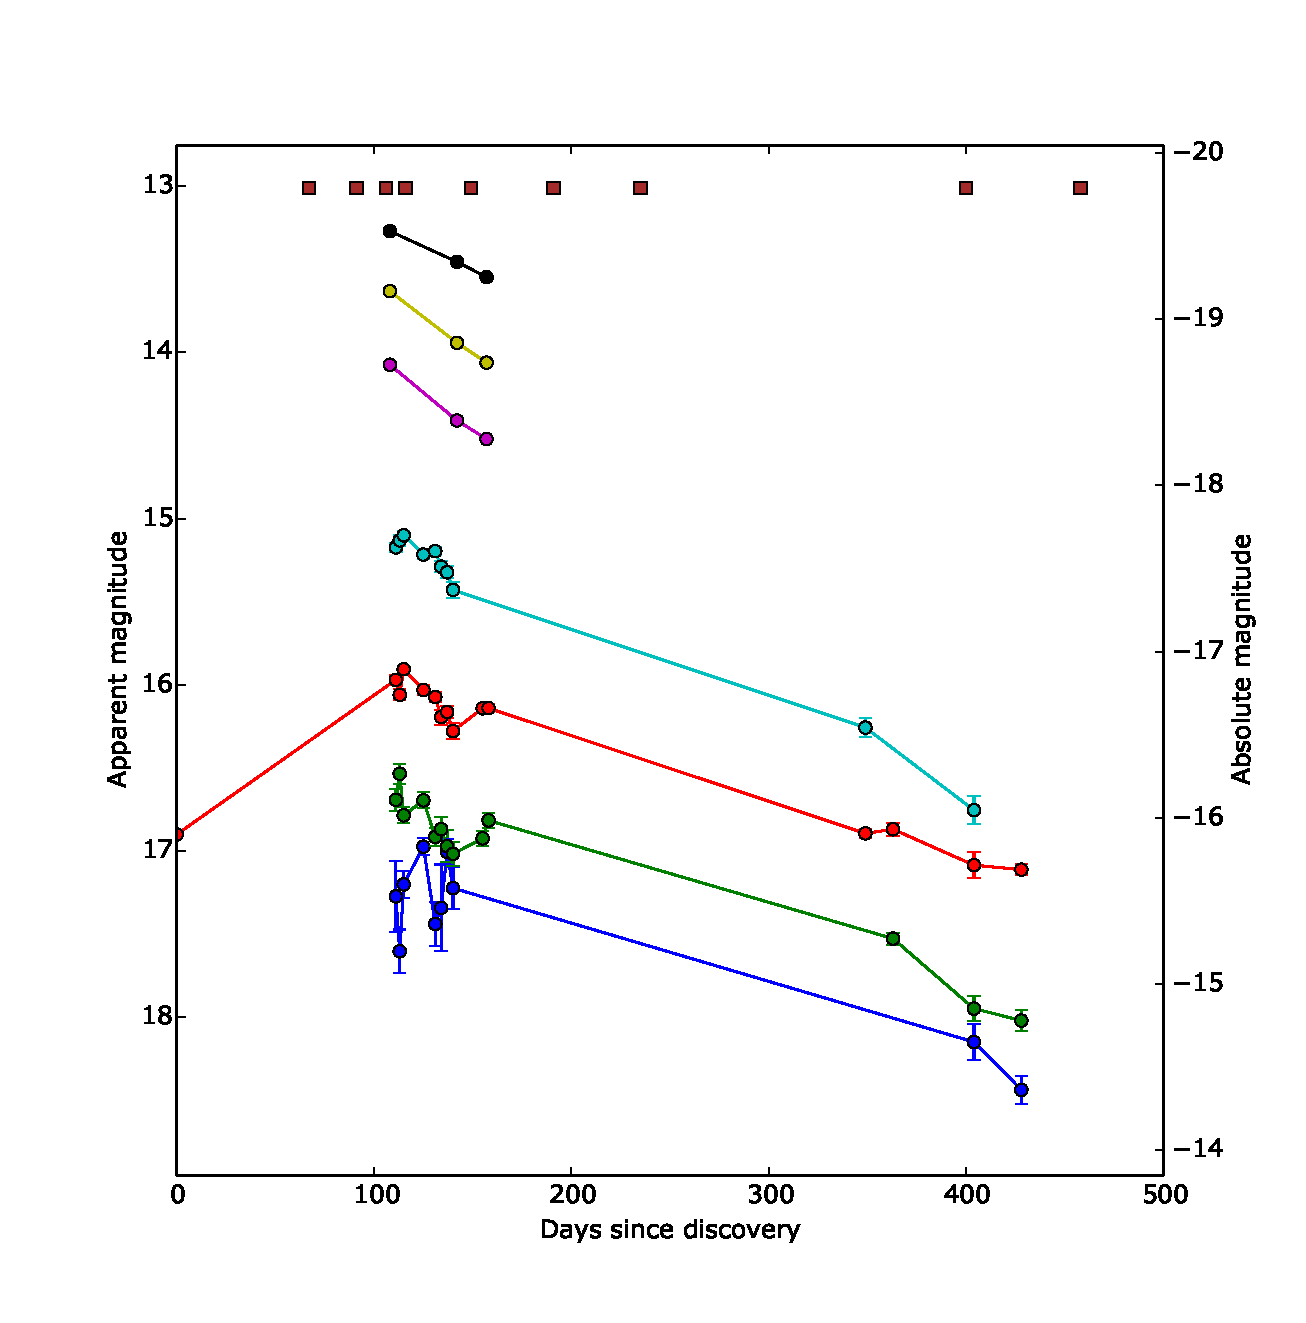
\includegraphics[width=\linewidth]{graphics/multi_full_spectra.eps}
  \caption{Photometric data for PSN J13522411. SLOTIS data in B, V, R, and I are plotted around ~100-160 days in blue, green, red, and cyan, respectively. The discovery magnitude is plotted in red at far left, and the Kuiper data are plotted at the far right. UKIRT data in J, H, and K are plotted in magenta, yellow, and black, respectively. Dates for which spectral data are available are marked in brown at the top. All magnitudes have been corrected for Milky Way reddening.}
  \label{fig:curve}
\end{figure}

\subsection{Spectroscopy} \label{obs:spec}
Five high-resolution spectra were obtained using the Bluechannel (BC) spectrometer on the MMT with the 1200 line grating. Four of the spectra were taken during the first six months, while the fifth was taken much later. One early spectrum was obtained using the Multi Object Double Spectrograph \citep[MODS]{Bya00} on the LBT. Two broad spectra were obtained using the Kast spectrograph on the Lick 3-m Shane reflector \citep{Mil93}. Finally, one late-time spectrum was obtained using the Boller \& Chivens (B\&C) spectrograph on the Bok 90-inch telescope on Kitt Peak. All spectra were Doppler-corrected, and the broad spectra were also corrected for reddening. The full spectra are plotted in Fig. \ref{fig:full}, and details of the spectra are summarized in Table 4.

\begin{figure*}
  \centering
  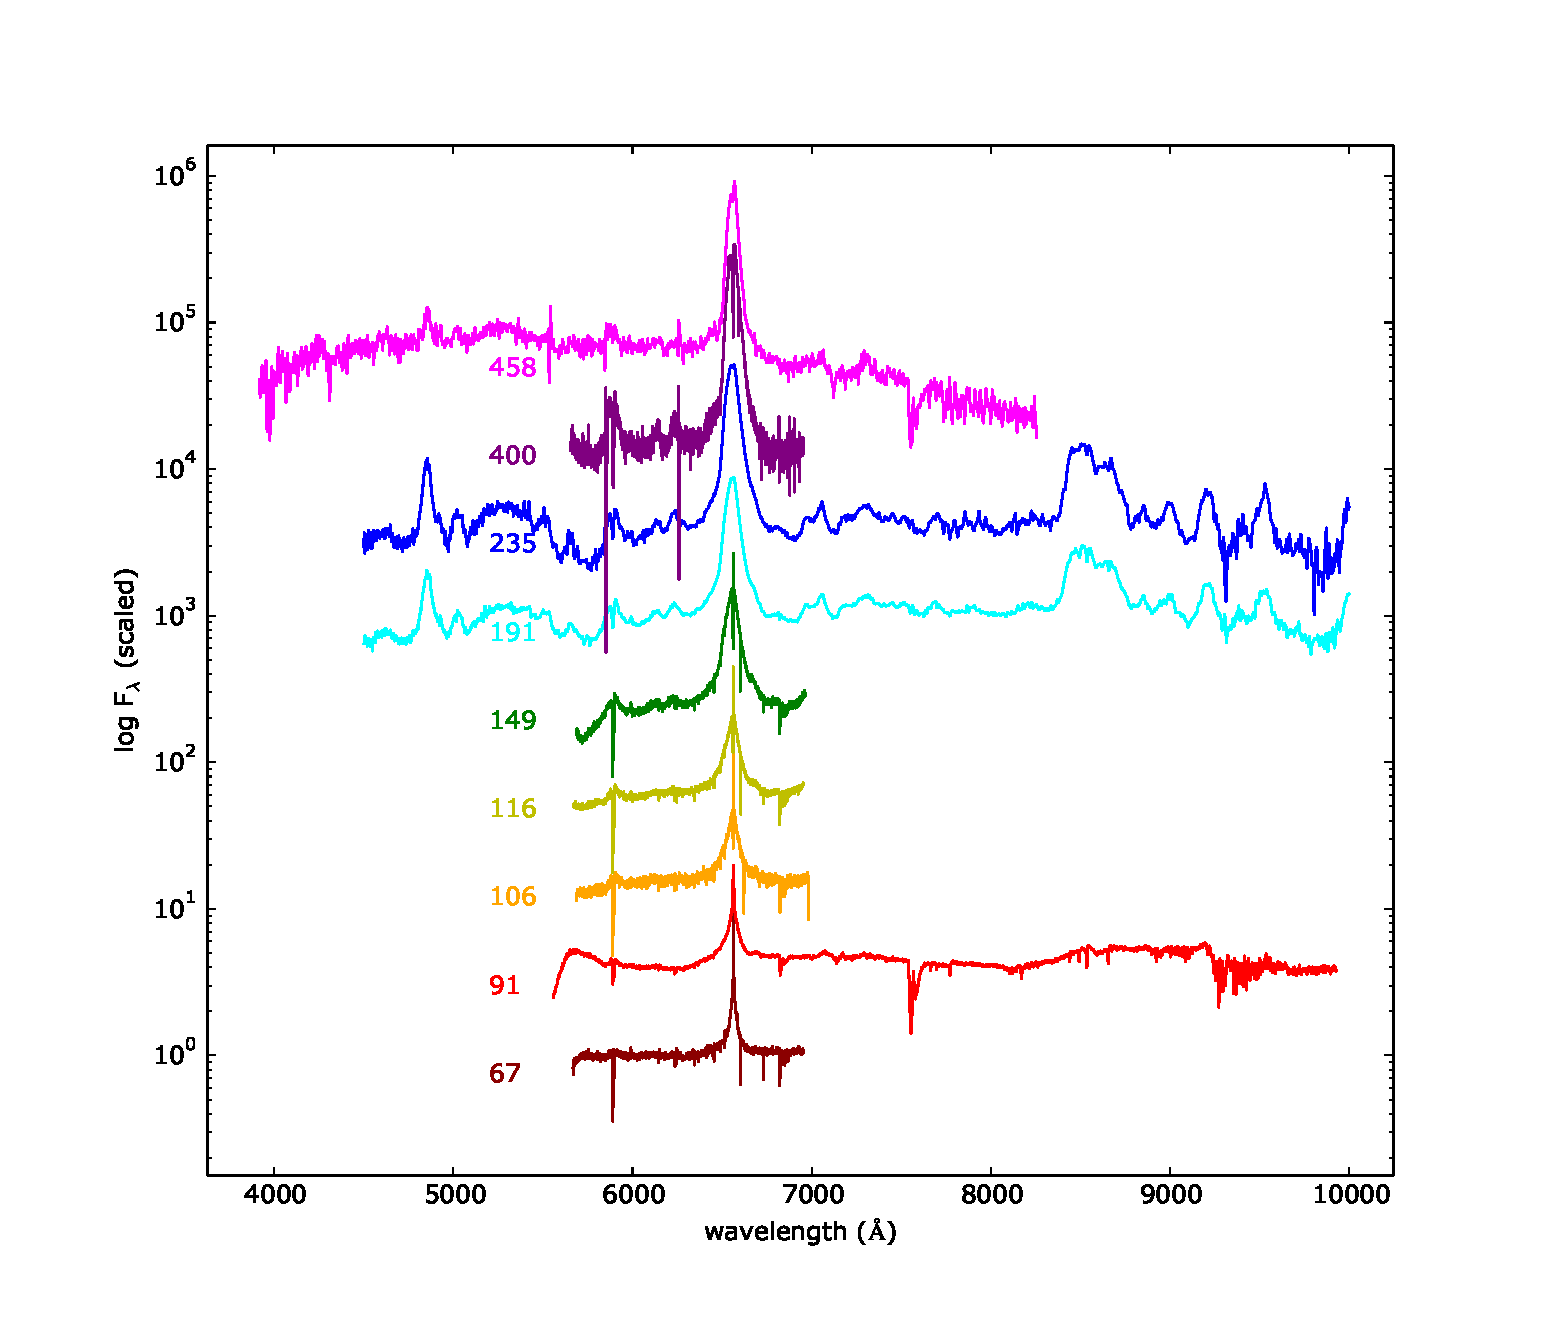
\includegraphics[width=18cm]{graphics/full.eps}[t!]
  \caption{All spectra of PSN J13522411, with early times at the bottom and later times at the top. The spectra have been normalized to the continuum at 6300 angstroms.}
  \label{fig:full}
\end{figure*}

%% Analysis
\section{Analysis} \label{analysis}
\subsection{Light curve} \label{analysis:curve}
\subsubsection{General features} \label{analysis:curve:gen}
The multiband light curves of PSN J13522411 are shown in Fig. \ref{fig:curve}. No data is available around the time of peak luminosity, so the exact peak date could be anywhere between $\sim10-50$ days. Likewise, the later portion of the light curve has a $>250$ d gap where no data was taken, so we can only assume that the decline during this period is basically linear. Despite the lack of sampling, it is clear that the SN is decaying quite slowly: in $\sim300$ days, the R brightness only decreased by $\sim1.1$ mag. This is much slower than would be expected from just the decay of radioactive cobalt, indicative of the strong interaction between the expanding shock and the CSM. For how long-lived it is, however, the SN is unusually dim. This may be due to extinction effects, either from the remaining cold CSM or from the host galaxy. In \S \ref{analysis:spec:red}, we use the sodium doublet to estimate reddening due to the host galaxy, concluding that $E(B-V)_{host} \approx 0.39$ mag. Assuming a similar reddening law to the Milky Way, this implies an additional $A_{R,host} = 0.585$ mag. We have not applied this correction to the light curve.

\subsubsection{Total emitted energy} \label{analysis:curve:energy}
If we assume that the R-band brightness is roughly equivalent to the bolometric magnitude, we can transform the R magnitudes into luminosities and integrate over time to get an estimate of the total radiated energy. Performing this calculation \citep{Are99}, we estimate the total emitted energy to be $\sim4 \times 10^{49}$ erg. Because we were not able to obtain any data during the period around maximum brightness, this value is probably a lower limit, putting the true value closer to $\sim10^{50}$ erg. In fact, using the correction factor we calculated in \S \ref{analysis:curve:gen}, our lower bound increases to $\sim7 \times 10^{49}$ erg, a more reasonable value for a SN IIn.

\subsection{Spectral evolution} \label{analysis:spec}
\subsubsection{General properties} \label{analysis:spec:gen}
Besides the H-alpha line discussed below, the spectra from Lick Observatory also show H-beta emission (weakly visible in Bok), bright emission lines from calcium in the near-infrared around $\sim8500$ angstroms, and other broad emission lines. The line at 5876 angstroms is bisected by strong absorption from the sodium D doublet. The H-alpha line also features several small absorption lines between $\sim6450-6525$ angstroms.

\begin{figure}
  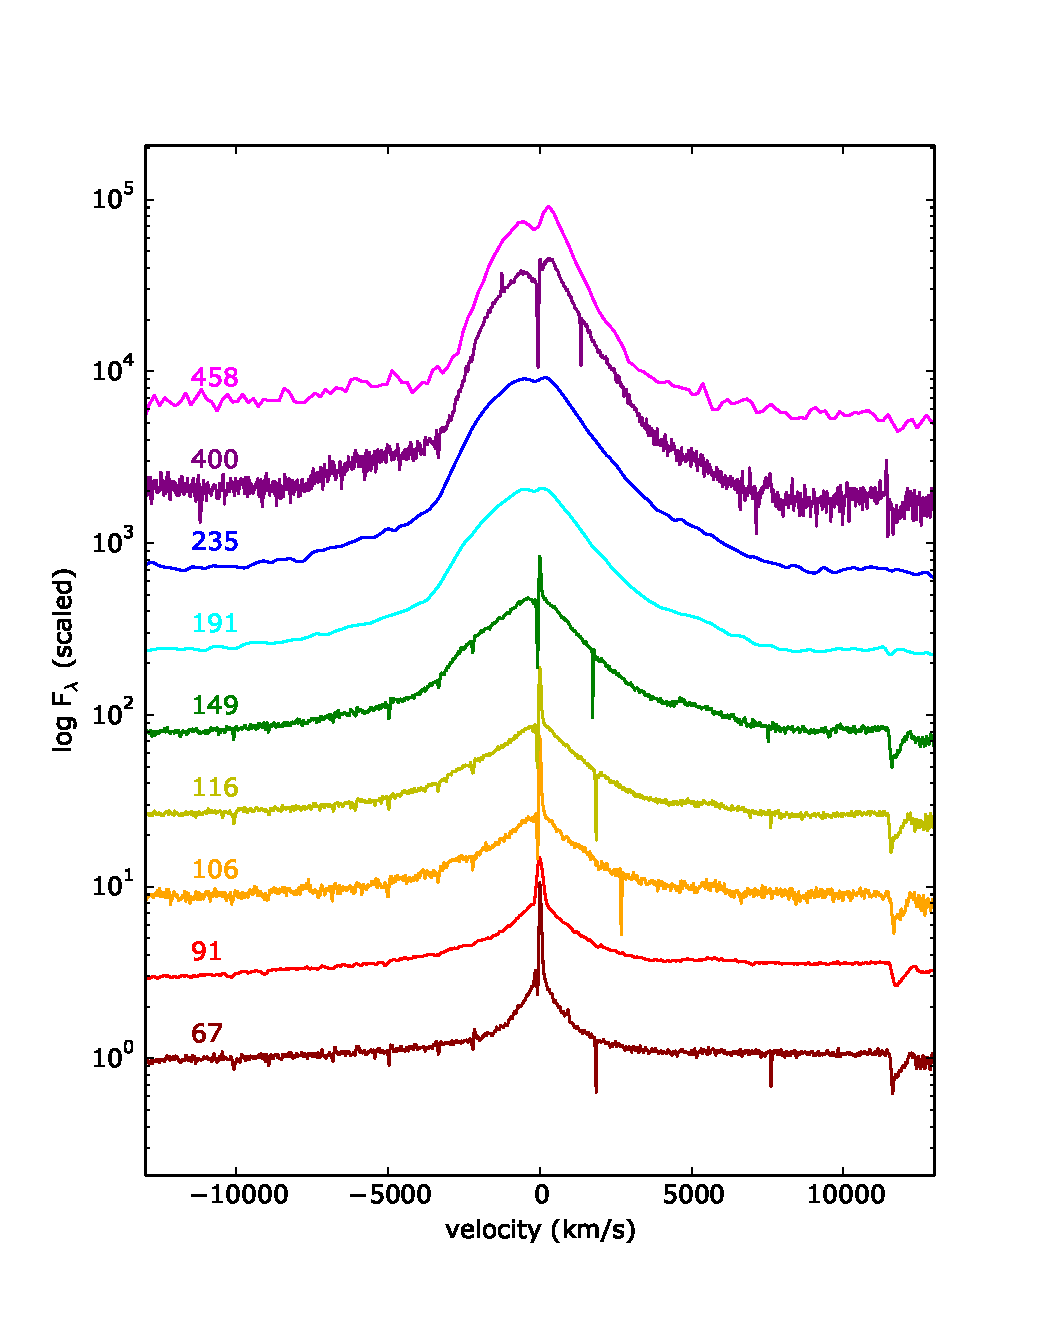
\includegraphics[width=\linewidth]{graphics/H_alpha.eps}
  \caption{Evolution of the H-alpha profile, normalized to the continuum at 6300 angstroms (12263 km/s). The sharp dips at $\sim$2000 km/s are bad pixels. The absorption features at the far right are telluric lines.}
  \label{fig:H-alpha}
\end{figure}

\subsubsection{Continuum} \label{analysis:spec:cont}
Initially, the continuum of PSN J13522411 was flat over the range of the MMT, while the LBT spectrum showed emission and absorption features in the near-infrared. Over the next few months, the continuum became more red, as seen in both the MMT and Lick spectra. This trend reversed sometime around 400 days after discovery, as the last MMT spectrum seems less diagonal, while the final spectrum from Bok has a blue continuum with a clear peak around $\sim5000$ angstroms, implying an effective temperature of $\sim5800$ K.

\subsubsection{H-alpha line evolution}\label{analysis:spec:line}
Refer to Fig. \ref{fig:H-alpha}. Initially, the broad H-alpha line is symmetrical with a FWHM of $\sim1400$ km/s, with Lorentzian wings extending out to $\sim\pm5000$ km/s. On top of the broad component is a narrow P-Cygni feature, predominately emission, with a Gaussian FWHM of $\sim50$ km/s, about the resolution of the grating. As time progresses, the broad emission increases and becomes more humped until $\sim200$ d after discovery, after which the H-alpha flux starts to decrease; the overall profile, however, remains roughly symmetrical, indicating a relatively even distribution of CSM. The P-Cygni feature gradually transitions from mostly emission to almost all absorption, causing the appearance of a double peak in the broad emission. The FWHM of the broad emission rises rapidly, peaks around $\sim200$ d after discovery, then declines more gradually. At late times, very low, broad wings develop that extend out to $\sim 8000$ km/s. The peak-to-trough width of the P-Cygni feature remains roughly constant at $\sim70$ km/s.

\begin{figure}
  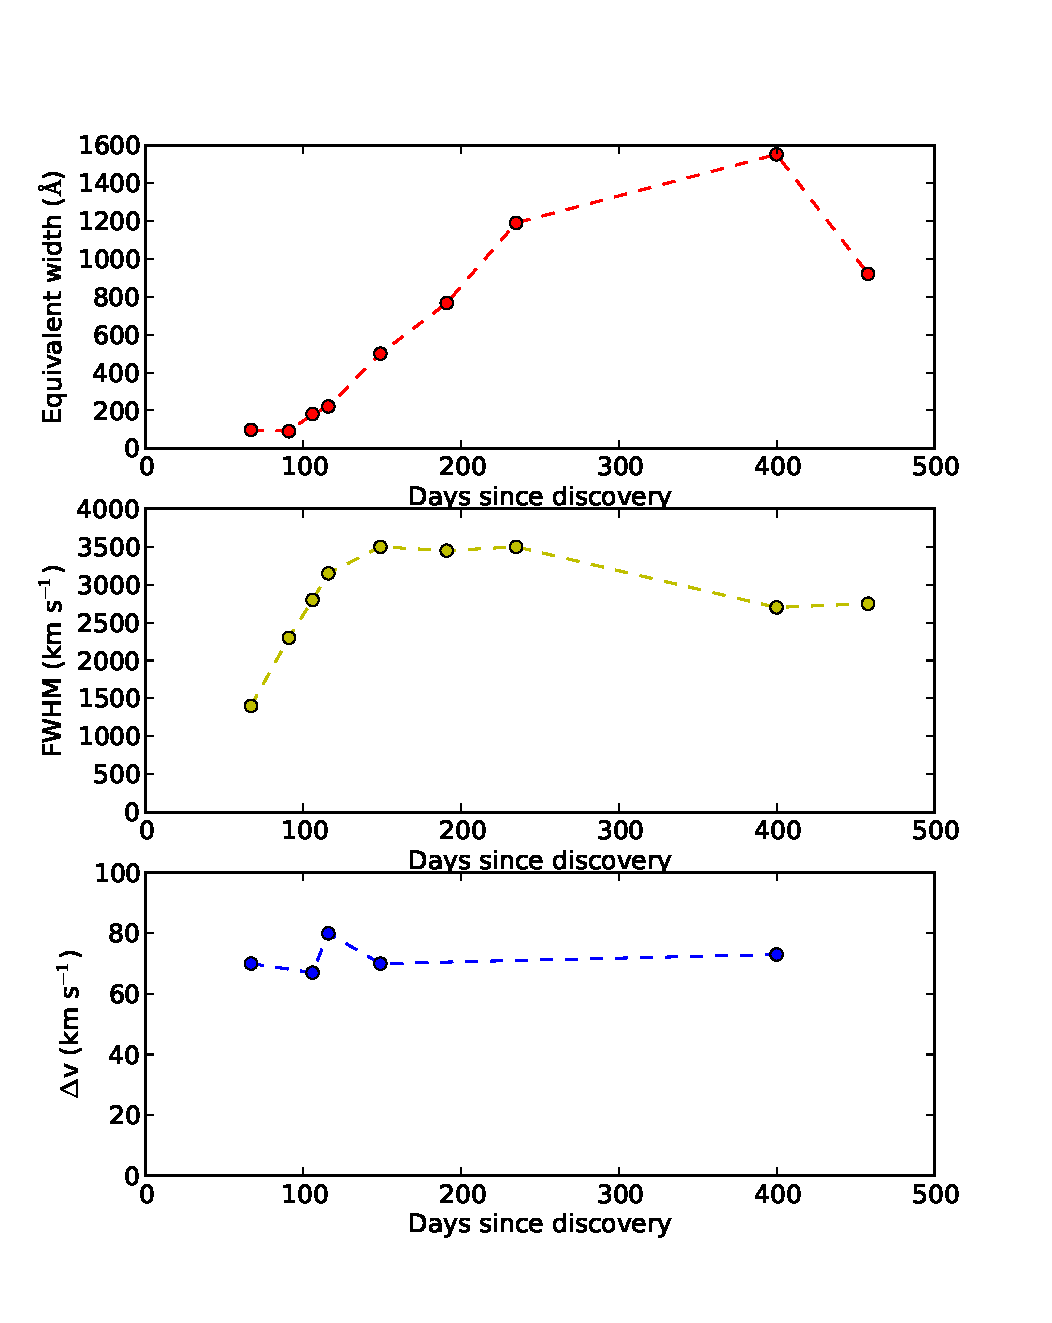
\includegraphics[width=\linewidth]{graphics/H-alpha_stats.eps}
  \caption{Properties of the H-alpha line, plotted over time. Top left: Equivalent width, measured between 6300-6800 angstroms. Top right: total flux of H-alpha emission, from the equivalent width measurements. Bottom left: FWHM of the broad H-alpha line. Bottom right: Peak-to-trough width of the P-Cygni profile in the high-resolution spectra.}
  \label{fig:stats}
\end{figure}

\begin{figure}
  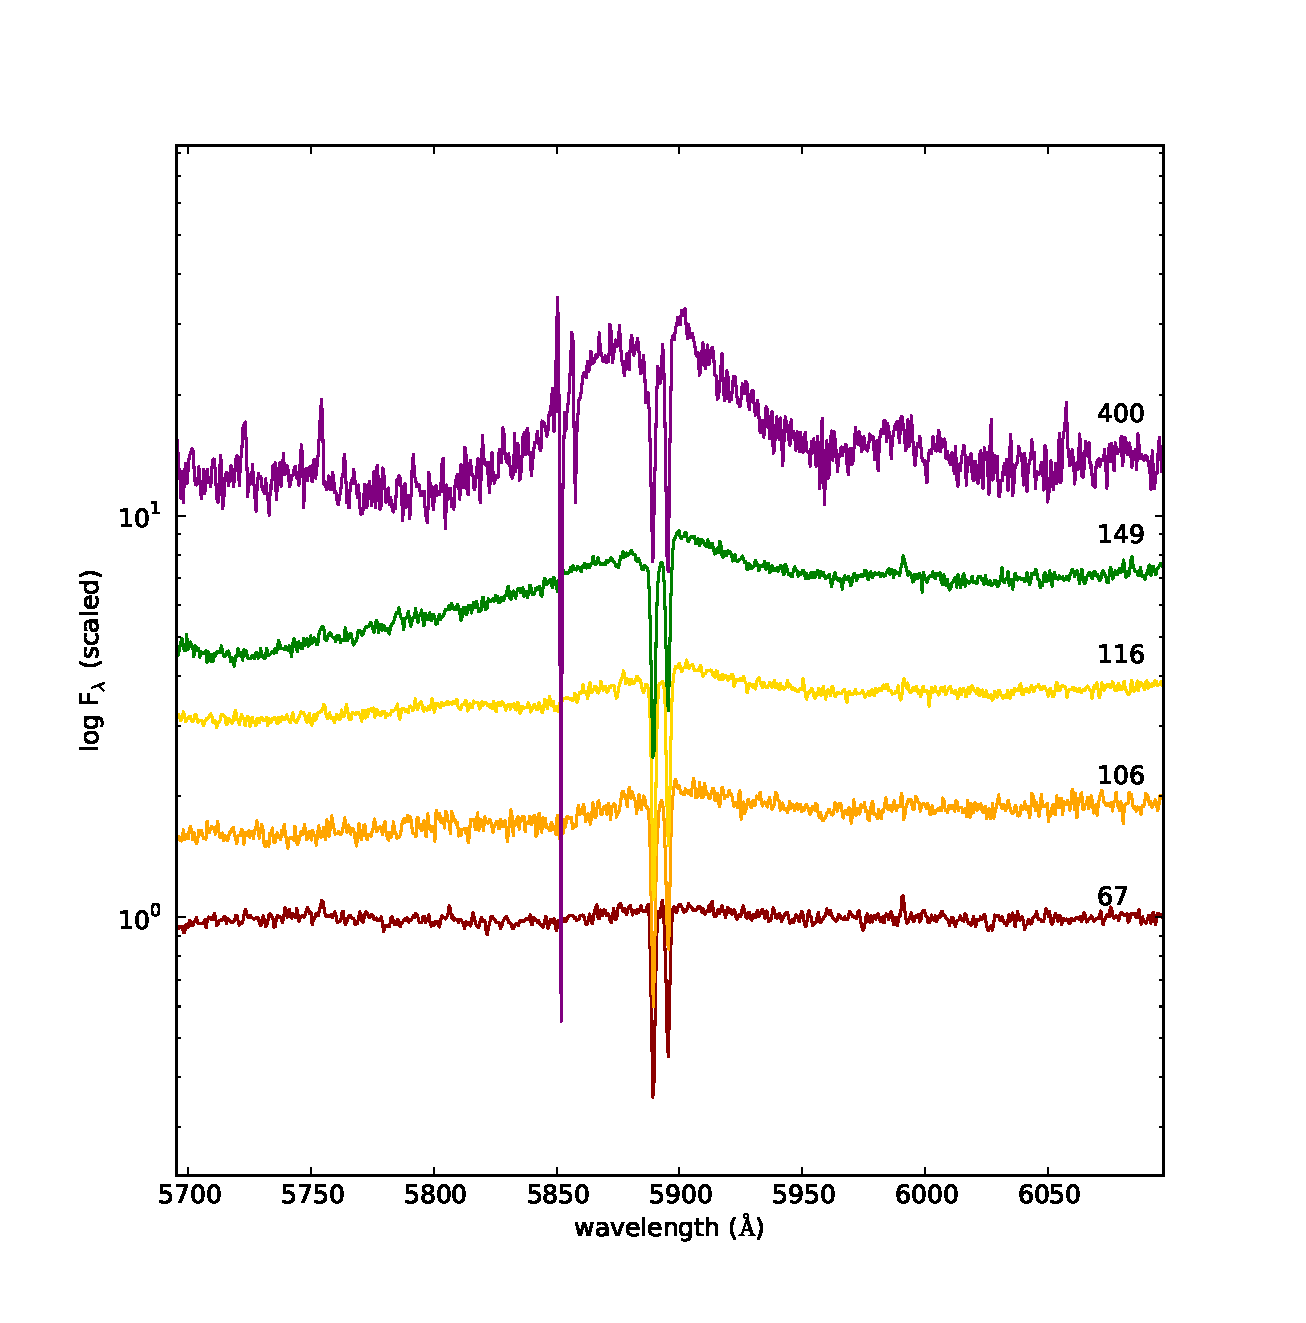
\includegraphics[width=\linewidth]{graphics/sodium.eps}
  \caption{Sodium emission with strong doublet absorption. The sharp spike at left in the top spectrum is likely a bad pixel.}
  \label{fig:sodium}
\end{figure}

\subsubsection{CSM properties} \label{analysis:spec:csm}
Taking half the FWHM as the velocity of the shock, we estimate the radius of the CSM with the following relation: $R_{CSM} \ge \frac{1}{2} \times v_{shock} \times \Delta t$. Plugging in $v_{shock} = 3500$ km/s and $\Delta t = 458 d$ (see Fig. \ref{fig:stats}, we determine the radius to be $\sim460 AU$. If we assume that the width of the P-Cygni feature indicates the velocity of the CSM, $v_{CSM} \approx 70$ km/s, we arrive at a lower age limit of $\sim31$ years; this may imply that the progenitor underwent little outward change during the later stages of nuclear burning. The low velocity of the pre-SN material indicates that the progenitor was most likely a red or yellow supergiant \citep{Smi15}, rather than a Wolf-Rayet star or LBV. That the H-alpha emission remains as bright as it does at such late times and large distances suggests that the stellar wind was relatively dense; the exact value will be determined at a later time.

\subsubsection{Host reddening} \label{analysis:spec:red}
Using the Na D doublet, shown in close-up in Fig. \ref{fig:sodium}, we can estimate the amount of reddening due to dust in the host galaxy \citep{Poz12}. Measuring the equivalent width of each line and comparing to the respective chart of equivalent width vs. reddening, we estimate $E(B-V)_{host} \approx 0.39$ mag. We have not applied this correction to either the light curve or the spectra, but we discuss the implications for the total energy in \S \ref{analysis:curve:energy}.

%% Conclusion
\section{Conclusion} \label{conclusion}
We obtained photometry and spectra of PSN J13522411 covering the early and later portions of the SN's decline. By integrating the light curve, we estimate the total radiated energy at $\sim10^{50}$ erg. From the spectral data, we infer that the CSM is a dense, roughly symmetrical stellar wind that had been blowing for at least the last 30 years before the explosion. We also infer from the velocity of the stellar wind that the progenitor was likely a red or yellow supergiant. Due to time constraints, we have not yet completed our analysis of this SN. In the coming weeks, we plan to determine the mass and distribution of the CSM and the total energy of the explosion.

%% Acknowledgements
\section{Acknowledgements}
Special thanks goes to Dr. Jennifer Andrews for her assistance with data management and reduction. Also to Dr. Peter Milne, Principal Investigator for the Super-LOTIS robotic telescope, for his advice on working with the SLOTIS data.

%% Bibliography
\begin{thebibliography}{}
\bibitem[Aretxaga et al.(1999)]{Are99} Aretxaga I. et al., 1999, MNRAS, 309, 343
\bibitem[Byard and O'Brien(2000)]{Bya00} Byard P. L., O'Brien T. P., 2000, Proc. SPIE, 4008, 934
\bibitem[Filippenko(1997)]{Fil97} Filippenko A. V., 1997, ARA\&A, 35, 309
\bibitem[Fontaine et al.(2014)]{Fon14} Fontaine G. et al., 2014, ASP Conference Series, 481, 19
\bibitem[Fransson et al.(2015)]{Fra15} Fransson, C. et al., 2015, The Astrophysical Journal Letters, 806, L19
\bibitem[Hodgkin et al.(2009)]{Hod09} Hodgkin S. T. et al., 2009, MNRAS 394, 675
\bibitem[Miller and Stone(1993)]{Mil93} Miller J. S., Stone R. P. S., 1993, Lick Obs. Tech. Rep. 66, Lick Obs., Santa Cruz
\bibitem[Poznanski et al.(2012)]{Poz12} Poznanski D. et al., 2012, MNRAS, 426, 1465
\bibitem[Smith et al.(2015)]{Smi15} Smith N. et al., 2015, MNRAS, 449, 1876
\bibitem[Williams et al.(2008)]{Wil08} Williams G. G. et al., 2008, AIP Conference Proceedings, 1000, 535
\end{thebibliography}

\end{document}
